
%----------------------------------------------------------------------------------------%
% START LaTeX preamble

% define document type, font and paper size
\documentclass[11pt,a4paper]{article}

%----------------------------------------------------------------------------------------%
% IMPORT LaTeX packages

\usepackage{inputenc}
\usepackage[ngerman, english]{babel}
\usepackage{csquotes}
\usepackage{amsmath}
\usepackage{amssymb}
\usepackage{amsfonts}
\usepackage{graphicx}
\usepackage{wrapfig}
\usepackage[margin=1.25in]{geometry}
\usepackage{pdfpages}
\usepackage{listings}
\usepackage{setspace}
\usepackage{systeme}
\usepackage{mdframed}
\newcommand{\mathsym}[1]{{}}
\newcommand{\unicode}[1]{{}}




%----------------------------------------------------------------------------------------%
% IMPORT LaTeX packages to manange bibliography

% MLA, APA, or IEEE? - https://www.overleaf.com/learn/latex/Biblatex_citation_styles
\usepackage[style=apa, backend=biber]{biblatex}
\addbibresource{bibliography.bib}

%----------------------------------------------------------------------------------------%
% DEFINE header values

% define the cover page values
\title
{
    Homework 02 - Introduction to Systems of Linear Equations
}
\author
{    
    Bruno Gonz{\' a}lez Soria (A01169284)  \\
    Antonio Osamu Katagiri Tanaka (A01212611) \\
    Jos{\' e} Ivan Aviles Castrillo (A01749804) \\
    Jes{\' u}s Alberto Mart{\' i}nez Espinosa (A01750270) \\
    Katya Michelle Aguilar P{\' e}rez (A01750272) \\
    \\
    Instructor: Ph.D Daniel L{\' o}pez Aguayo
}
\date{\today}

%----------------------------------------------------------------------------------------%
% USER-DEFINED commands

% Keywords command
\providecommand{\keywords}[1]
{
    \\
    \\
    \small
    \textbf{\textit{Keywords:}} #1
}

%----------------------------------------------------------------------------------------%

\begin{document}
\setlength\parindent{0pt} % Set noindent for entire file

%----------------------------------------------------------------------------------------%
% CREATE the 1st page (cover page)

\maketitle

%----------------------------------------------------------------------------------------%
% DEFINE the abstract text & keywords

%\begin{abstract}
%    \emph
%    {
%        Lorem ipsum dolor sit amet, consectetur adipiscing elit, sed do eiusmod tempor incididunt ut labore et dolore magna aliqua. Ut enim ad minim veniam, quis nostrud exercitation ullamco laboris nisi ut aliquip ex ea commodo consequat. Duis aute irure dolor in reprehenderit in voluptate velit esse cillum dolore eu fugiat nulla pariatur. Excepteur sint occaecat cupidatat non proident, sunt in culpa qui officia deserunt mollit anim id est laborum.
%    }
%    \keywords{Lorem, ipsum, dolor, sit, amet}
%\end{abstract}
\clearpage

%----------------------------------------------------------------------------------------%
% CREATE a table of contents in a new page

%\tableofcontents
%\clearpage

%----------------------------------------------------------------------------------------%
% CREATE a list of figures and a list of tables in a new page

%\listoffigures
%\listoftables
%\clearpage

%----------------------------------------------------------------------------------------%
% DOCUMENT body starts here

%----------------------------------------------------------------------------------------%
%Append the HW's exercises
\includepdf[page=-]{HW2}

%----------------------------------------------------------------------------------------%
\section{Answer to Problem I}\label{sec:P01} %Osamu

I.1\\
\(x-\text{$\pi $y}+\sqrt[3]{5}z=0\) is a linear equation\\

I.2\\
\(x^2+y^2+z^2=1\) is NOT a linear equation\\
The variables shall occur only to the first power.\\

I.3\\
\(x^{-1}+7y+z=\)\(\left(\text{Sin}\left[\frac{\pi }{9}\right]\right)^2\) is NOT a linear equation\\
The variables shall occur only to the first power.\\

I.4\\
\(x+7y+z=\text{Sin}\left[\frac{\pi }{9}\right]\) is a linear equation\\

I.5\\
\(3\text{Cos}[x]-4y+z=\sqrt{3}\) is NOT a linear equation\\
Linear equations shall not contain products, reciprocals or other functions of the variables.\\

I.6\\
\(\text{Cos}[3]x-4y+z=\sqrt{3}\) is a linear equation

\clearpage
%----------------------------------------------------------------------------------------%
\section{Answer to Problem II}\label{sec:P02} %Osamu

II.7\\
\begin{doublespace}
\noindent\(\pmb{\text{ContourPlot}[\{x + y \text{==} 0, 2*x + y \text{==} 3\}, \{x, 2, 4\}, \{y, -4, -2\},}\\
\pmb{\text{ContourStyle}\to \{\text{Blue},\text{Orange}\}]}\\
\pmb{\text{(*}}\\
\pmb{
\begin{array}{ll}
 \{ & 
\begin{array}{ll}
 x+y & =0 \\
 2x+y & =3 \\
\end{array}
 \\
\end{array}
\Rightarrow \left(
\begin{array}{ccc}
 1 & 1 & 0 \\
 2 & 1 & 3 \\
\end{array}
\right)\Rightarrow R_2-2R_1\Rightarrow \left(
\begin{array}{ccc}
 1 & 1 & 0 \\
 0 & -1 & 3 \\
\end{array}
\right)\Rightarrow 
\begin{array}{ll}
 \{ & 
\begin{array}{ll}
 x+y & =0 \\
 -y & =3 \\
\end{array}
 \\
\end{array}
}\\
\boxed{\pmb{y=-3}}\\
\pmb{}\\
\pmb{x+y=0}\\
\pmb{x=-(-3)}\\
\boxed{\pmb{x=3}}\\
\pmb{\text{*)}}\\
\pmb{\text{Solve}[\{x + y \text{==} 0,2*x + y \text{==} 3\}, \{x,y\}]}\)
\end{doublespace}
\begin{figure}[!htbp]
\includegraphics[width=0.60\textwidth]{img/h2_gr1.eps}
%\includegraphics[width=0.60\textwidth]{img/ii_7.png}
\end{figure}
As shown in the plot, the system has one solution.\\
\begin{doublespace}
\noindent\(\{\{x\to 3,y\to -3\}\}\)
\end{doublespace}

\clearpage

II.8\\
\begin{doublespace}
\noindent\(\pmb{\text{ContourPlot}[\{x - 2*y \text{==} 7, 3*x + y \text{==} 7\}, \{x, 2, 4\}, \{y, -3, -1\},}\\
\pmb{\text{ContourStyle}\to \{\text{Blue},\text{Orange}\}]}\\
\pmb{\text{(*}}\\
\pmb{
\begin{array}{ll}
 \{ & 
\begin{array}{ll}
 x-2y & =7 \\
 3x+y & =7 \\
\end{array}
 \\
\end{array}
\Rightarrow \left(
\begin{array}{ccc}
 1 & -2 & 7 \\
 3 & 1 & 7 \\
\end{array}
\right)\Rightarrow R_2-3R_1\Rightarrow \left(
\begin{array}{ccc}
 1 & -2 & 7 \\
 0 & 7 & -14 \\
\end{array}
\right)\Rightarrow 
\begin{array}{ll}
 \{ & 
\begin{array}{ll}
 x-2y & =7 \\
 7y & =-14 \\
\end{array}
 \\
\end{array}
}\\
\boxed{\pmb{y=-2}}\\
\pmb{}\\
\pmb{x-2y=7}\\
\pmb{x=7+2(-2)}\\
\boxed{\pmb{x=3}}\\
\pmb{\text{*)}}\\
\pmb{\text{Solve}[\{x - 2*y \text{==} 7,3*x + y \text{==} 7\}, \{x,y\}]}\)
\end{doublespace}
\begin{figure}[!htbp]
\includegraphics[width=0.60\textwidth]{img/h2_gr2.eps}
%\includegraphics[width=0.60\textwidth]{img/ii_8.png}
\end{figure}
As shown in the plot, the system has one solution.\\
\begin{doublespace}
\noindent\(\{\{x\to 3,y\to -2\}\}\)
\end{doublespace}

\clearpage

II.9\\
\begin{doublespace}
\noindent\(\pmb{\text{ContourPlot}[\{3*x - 6*y \text{==} 3, -x + 2*y \text{==} 1\}, \{x, -3.125, 4.5\}, \{y, -1.75, 1.75\},}\\
\pmb{\text{ContourStyle}\to \{\text{Blue},\text{Orange}\}]}\\
\pmb{\text{(*}}\\
\pmb{
\begin{array}{ll}
 \{ & 
\begin{array}{ll}
 3x-6y & =3 \\
 -x+2y & =1 \\
\end{array}
 \\
\end{array}
\Rightarrow \left(
\begin{array}{ccc}
 3 & -6 & 3 \\
 -1 & 2 & 1 \\
\end{array}
\right)\Rightarrow R_2+\frac{1}{3}R_1\Rightarrow \left(
\begin{array}{ccc}
 3 & -6 & 3 \\
 0 & 0 & 2 \\
\end{array}
\right)\Rightarrow 
\begin{array}{ll}
 \{ & 
\begin{array}{ll}
 3x-6y & =3 \\
 0 & =2 \\
\end{array}
 \\
\end{array}
}\\
\boxed{\pmb{\text{no } \text{solution}}}\\
\pmb{\text{*)}}\\
\pmb{\text{Solve}[\{ 3*x - 6*y \text{==} 3,\text{  }-x + 2*y \text{==} 1\}, \{x,y\}]}\)
\end{doublespace}
\begin{figure}[!htbp]
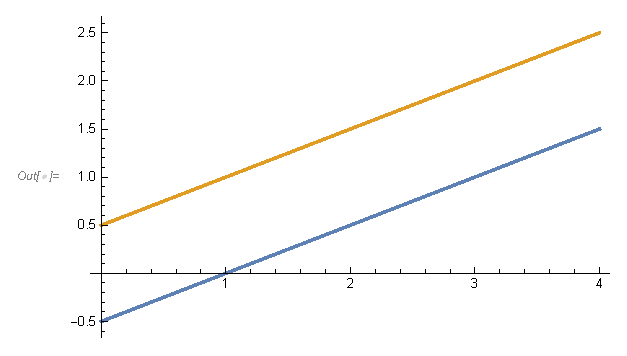
\includegraphics[width=0.60\textwidth]{img/h2_gr3.eps}
%\includegraphics[width=0.60\textwidth]{img/ii_9.png}
\end{figure}
As shown in the plot, the system has no solution.\\
\begin{doublespace}
\noindent\(\{\}\)
\end{doublespace}

\clearpage
%----------------------------------------------------------------------------------------%
\section{Answer to Problem III}\label{sec:P03}
10. \\
\\\[
\systeme*{x-y+z=0,2y-z=1,3z=-1}
\]
  
From last equation \pmb{ z=-1/3}, therefore 2y+1/3=1 then \pmb{ y=1/3}. For first equation It obtains\pmb{  x}=1/3+1/3=\pmb{ 2/3}\\
\\
\\
\\
11.\\
\\\[
\systeme*{x_1+2x_2+3x_3=0,-5x_2+2x_3=0,4x_3=0}
\]

From last equation \pmb{ x3=0}. Using second equation we obtain\pmb{  x2}=(2(0))/5\pmb{ =0} then for first equation \pmb{ x1}=-3(0)-2(0)=\pmb{ 0\\
\\
}
\\12. \\
\\\[
\systeme*{x_1+x_2-x_3-x_4=1,x_2+x_3+x_4=0,x_3-x_4=0,x_4=1}
\]

From last equation \pmb{ x4=1} then \pmb{ x3=1} therefore from second equation\pmb{  x2}=-1-1\pmb{ =-2}. Finally from first equation \pmb{ x1}=1+2+1+1\pmb{
=5}\\


\begin{doublespace}
\noindent\(\pmb{\text{}}\)
\end{doublespace}


\clearpage
%----------------------------------------------------------------------------------------%
\section{Answer to Problem IV}\label{sec:P04}



\clearpage
%----------------------------------------------------------------------------------------%
\section{Answer to Problem V}\label{sec:P05}



\clearpage
%----------------------------------------------------------------------------------------%
\section{Answer to Problem VI}\label{sec:P06}



\clearpage
%----------------------------------------------------------------------------------------%
\section{Answer to Problem VII}\label{sec:P07}



\clearpage
%----------------------------------------------------------------------------------------%
\section{Answer to Problem VIII}\label{sec:P08} %Osamu

\begin{doublespace}
\noindent\(\\
\pmb{
\begin{array}{ll}
 \{ & 
\begin{array}{ll}
 \text{kx}+y & =-2 \\
 2x-2y & =4 \\
\end{array}
 \\
\end{array}
\Rightarrow \left(
\begin{array}{ccc}
 k & 1 & -2 \\
 2 & -2 & 4 \\
\end{array}
\right)\Rightarrow \frac{1}{k}R_1\Rightarrow \left(
\begin{array}{ccc}
 1 & \frac{1}{k} & -\frac{2}{k} \\
 2 & -2 & 4 \\
\end{array}
\right)\Rightarrow R_2-2R_1\Rightarrow
}
\pmb{
\left(
\begin{array}{ccc}
 1 & \frac{1}{k} & -\frac{2}{k} \\
 0 & -\frac{2 (1+k)}{k} & 4+\frac{4}{k} \\
\end{array}
\right)\Rightarrow }
\pmb{-\frac{k}{2 (1+k)}R_2\Rightarrow \left(
\begin{array}{ccc}
 1 & \frac{1}{k} & -\frac{2}{k} \\
 0 & 1 & -2 \\
\end{array}
\right)\Rightarrow R_1-\frac{1}{k}R_2\Rightarrow \left(
\begin{array}{ccc}
 1 & 0 & 0 \\
 0 & 1 & -2 \\
\end{array}
\right)}\\
\pmb{
\boxed{
\begin{array}{c}
 x=0 \\
 y=-2; \text{for } \text{all } k \\
\end{array}
}
}\)
\end{doublespace}

Verification using Mathematica:

\begin{doublespace}
\noindent\(\pmb{A=\left(
\begin{array}{ccc}
 k & 1 & -2 \\
 2 & -2 & 4 \\
\end{array}
\right);}\\
\pmb{\text{RowReduce}[A];}\\
\pmb{\text{MatrixForm}[\%]}\\
\pmb{\text{Solve}[\{k*x+y==-2,2x-2y==4\},\{x,y\}]}\\
\pmb{\text{xMin}=-3;}\\
\pmb{\text{xMax}=2;}\\
\pmb{\text{ContourPlot3D}[\{k*x+y==-2,2x-2y==4\},\{x,\text{xMin},\text{xMax}\},\{y,\text{xMin},\text{xMax}\},}\\
\pmb{\{k,\text{xMin},\text{xMax}\},\text{Axes}\to \text{True},\text{AxesLabel}\to \{x,y,z\},\text{PlotLegends}\to \text{{``}Expressions{''}}]}\)
\end{doublespace}

\begin{doublespace}
\noindent\(\left(
\begin{array}{ccc}
 1 & 0 & 0 \\
 0 & 1 & -2 \\
\end{array}
\right)\)
\end{doublespace}

\begin{doublespace}
\noindent\(\{\{x\to 0,y\to -2\}\}\)
\end{doublespace}

\clearpage
%----------------------------------------------------------------------------------------%
\section{Answer to Problem IX}\label{sec:P09}

First the Condition for a single point of intersection of three planes is: Rc=Rd=3\\
Rc is the Matrix Rank and Rd is the Extended Matrix Rank\\
To accomplish this, we must find a matrix that no row or column can be put as a linear combination of the rest.\\
\\
one example of this is:\\
\\
\[
\systeme*{x+2 y+3 z=7,3 x+5 y+7 z=21,4 x+6 y+5 z=26}
\]

The matrix is

\begin{doublespace}
\noindent\(\pmb{A=\{\{1,2,3\},\{3,5,7\},\{4,6,5\}\}}\)
\end{doublespace}

\begin{doublespace}
\noindent\(\{\{1,2,3\},\{3,5,7\},\{4,6,5\}\}\)
\end{doublespace}

We can see that no row or column can be put as a linear equation of the rest, this means that it\'{ }s not posible to reduce the matrix in ceros and ones if you sum or rest the rows\\
\\
The extended matrix is

\begin{doublespace}
\noindent\(\pmb{B=\{\{1,2,3,7\},\{3,5,7,21\},\{4,6,5,26\}\}}\)
\end{doublespace}

\begin{doublespace}
\noindent\(\{\{1,2,3,7\},\{3,5,7,21\},\{4,6,5,26\}\}\)
\end{doublespace}

The ranks are:

\begin{doublespace}
\noindent\(\pmb{\text{MatrixRank}[A]}\)
\end{doublespace}

\begin{doublespace}
\noindent\(3\)
\end{doublespace}

\begin{doublespace}
\noindent\(\pmb{\text{MatrixRank}[B]}\)
\end{doublespace}

\begin{doublespace}
\noindent\(3\)
\end{doublespace}

For this we can infer that the three planes intersect in a single point.\\
We can plot to prove that:

\begin{doublespace}
\noindent\(\pmb{\text{}}\)
\end{doublespace}


\pmb{\text{ContourPlot3D}[\{x+2 y+3 z==7,3 x+5 y+7 z==21,4 x+6 y+5 z==26\},\{x,5,8\},\{y,-2,1\}\\
\\,\{z,-3,1\}]}


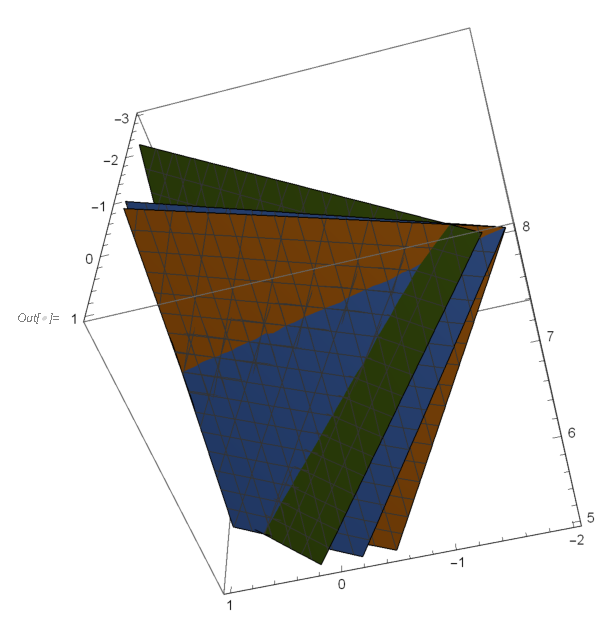
\includegraphics{img/h3_gr1.eps}

Also we can prove it if we solve the System:

\begin{doublespace}
\noindent\(\pmb{\text{Solve}[\{x+2 y+3 z==7,3 x+5 y+7 z==21,4 x+6 y+5 z==26\}]}\)
\end{doublespace}

\begin{doublespace}
\noindent\(\left\{\left\{x\to \frac{23}{3},y\to -\frac{4}{3},z\to \frac{2}{3}\right\}\right\}\)
\end{doublespace}

For this the example is a system of planes that intersect in one single point


\clearpage
%----------------------------------------------------------------------------------------%
\section{Answer to Problem X}\label{sec:P10}



\clearpage
%----------------------------------------------------------------------------------------%
\section{Answer to Problem XI}\label{sec:P11}



\clearpage
%----------------------------------------------------------------------------------------%
\section{Answer to Optional Problem 1}\label{sec:P12} %Osamu

Consider the following matrix\\
A=\(\left(
\begin{array}{ccc}
 \pi  & \pi  & \pi  \\
 \pi ^2 & \pi ^2 & \pi ^2 \\
 \pi ^3 & \pi ^3 & \pi ^3 \\
\end{array}
\right)\)\\
1. Find the reduced row echelon from of A; then find the rank of A.\\
2. How can you enter in Mathenatica (in one line) the matrix A? (without typing every entry!). Hint: Consider the Table command.\\
3. Now generalize the result as follows: let X be the following arbitrary square matrix of size n, where c is any non-zero number. Compute the rank
of X.\\
X=\(\left(
\begin{array}{cccc}
 c & c & \cdots  & c \\
 c^2 & c^2 & \cdots  & c^2 \\
 \vdots  & \vdots  & \vdots  & \vdots  \\
 c^n & c^n & \cdots  & c^n \\
\end{array}
\right)\)

\begin{doublespace}
Optional 1.1
\noindent\(\\
\pmb{\text{Print}[\text{{``}RowReduce[A]={''}} \text{MatrixForm}[\text{RowReduce}[A]]]}\\
\pmb{\text{Print}[\text{{``}MatrixRank[A]={''}}]}\\
\pmb{\text{MatrixRank}[A]}\)
\end{doublespace}


\noindent\(\boxed{\text{RowReduce[A]=} \left(
\begin{array}{ccc}
 1 & 1 & 1 \\
 0 & 0 & 0 \\
 0 & 0 & 0 \\
\end{array}
\right)}\)

\noindent\(\boxed{\text{MatrixRank[A]=}\)
\noindent\(1}\)

\begin{doublespace}
Optional 1.2\\
\noindent\(\boxed{\pmb{A=\text{Table}[\text{Pi}{}^{\wedge}i,\{i,1,3\},\{j,1,3\}];}}\)

\noindent\(\pmb{\text{MatrixForm}[A]}\)
\end{doublespace}

\begin{doublespace}
\noindent\(\left(
\begin{array}{ccc}
 \pi  & \pi  & \pi  \\
 \pi ^2 & \pi ^2 & \pi ^2 \\
 \pi ^3 & \pi ^3 & \pi ^3 \\
\end{array}
\right)\)
\end{doublespace}

Optional 1.3
\begin{mdframed}
X=\(\left(
\begin{array}{cccc}
 c & c & \cdots  & c \\
 c^2 & c^2 & \cdots  & c^2 \\
 \vdots  & \vdots  & \vdots  & \vdots  \\
 c^n & c^n & \cdots  & c^n \\
\end{array}
\right)\Rightarrow\) \(\begin{array}{c}
 \frac{1}{X_{11}}R_1\rightarrow R_1 \\
 \frac{1}{X_{21}}R_2\rightarrow R_2 \\
 \vdots  \\
 \frac{1}{X_{\text{n1}}}R_n\rightarrow R_n \\
\end{array}
\Rightarrow\) \(\left(
\begin{array}{cccc}
 1 & 1 & \cdots  & 1 \\
 1 & 1 & \cdots  & 1 \\
 \vdots  & \vdots  & \vdots  & \vdots  \\
 1 & 1 & \cdots  & 1 \\
\end{array}
\right)\Rightarrow\)\\
\(\begin{array}{c}
 R_2-R_1\rightarrow R_2 \\
 R_3-R_1\rightarrow R_3 \\
 \vdots  \\
 R_n-R_1\rightarrow R_n \\
\end{array}
\Rightarrow\) \(\left(
\begin{array}{cccc}
 1 & 1 & \cdots  & 1 \\
 0 & 0 & \cdots  & 0 \\
 \vdots  & \vdots  & \vdots  & \vdots  \\
 0 & 0 & \cdots  & 0 \\
\end{array}
\right)\)
\end{mdframed}

\clearpage
%----------------------------------------------------------------------------------------%
\section{Answer to Optional Problem 2}\label{sec:P13} %Osamu

For what value(s) of k, if any, will the following system:\\
\(\begin{array}{ll}
 \{ & 
\begin{array}{ll}
 x+y+\text{kz} & =1 \\
 x+\text{ky}+z & =1 \\
 \text{kx}+y+z & =-2 \\
\end{array}
 \\
\end{array}\)\\
have\\
1. No solution\\
2. A unique solution\\
3. Infinitely many solutions\\
Hint. Find the reduced echelon form of the augmented matrix, then analyze different cases (beware of division by zero!).\\
\\
\(\begin{array}{ll}
 \{ & 
\begin{array}{ll}
 x+y+\text{kz} & =1 \\
 x+\text{ky}+z & =1 \\
 \text{kx}+y+z & =-2 \\
\end{array}
 \\
\end{array}
\Rightarrow\) \(\left(
\begin{array}{cccc}
 1 & 1 & k & 1 \\
 1 & k & 1 & 1 \\
 k & 1 & 1 & -2 \\
\end{array}
\right)\Rightarrow\) \(R_1\leftrightarrow R_3\Rightarrow\) \(\left(
\begin{array}{cccc}
 k & 1 & 1 & -2 \\
 1 & k & 1 & 1 \\
 1 & 1 & k & 1 \\
\end{array}
\right)\Rightarrow\) \(\frac{1}{k}R_1\rightarrow R_1\Rightarrow\) \(\left(
\begin{array}{cccc}
 1 & \frac{1}{k} & \frac{1}{k} & -\frac{2}{k} \\
 1 & k & 1 & 1 \\
 1 & 1 & k & 1 \\
\end{array}
\right)\Rightarrow\) \(\begin{array}{c}
 R_2-R_1\rightarrow R_2 \\
 R_3-R_1\rightarrow R_3 \\
\end{array}
\Rightarrow\) \(\left(
\begin{array}{cccc}
 1 & \frac{1}{k} & \frac{1}{k} & -\frac{2}{k} \\
 0 & k-\frac{1}{k} & 1-\frac{1}{k} & 1+\frac{2}{k} \\
 0 & 1-\frac{1}{k} & k-\frac{1}{k} & 1+\frac{2}{k} \\
\end{array}
\right)\Rightarrow\) \(R_1-\frac{1}{-1+k^2}R_2\rightarrow R_1\Rightarrow\) \(\left(
\begin{array}{cccc}
 1 & 0 & \frac{1}{1+k} & \frac{1+2k}{1-k^2} \\
 0 & k-\frac{1}{k} & 1-\frac{1}{k} & 1+\frac{2}{k} \\
 0 & 1-\frac{1}{k} & k-\frac{1}{k} & 1+\frac{2}{k} \\
\end{array}
\right)\Rightarrow\) \(\frac{k}{-1+k^2}R_2\rightarrow R_2\Rightarrow\) \(\left(
\begin{array}{cccc}
 1 & 0 & \frac{1}{1+k} & \frac{1+2k}{1-k^2} \\
 0 & 1 & \frac{1}{1+k} & \frac{2+k}{-1+k^2} \\
 0 & 1-\frac{1}{k} & k-\frac{1}{k} & 1+\frac{2}{k} \\
\end{array}
\right)\Rightarrow\) \(R_3-\left(1-\frac{1}{k}\right)R_2\rightarrow R_3\Rightarrow\) \(\left(
\begin{array}{cccc}
 1 & 0 & \frac{1}{1+k} & \frac{1+2k}{1-k^2} \\
 0 & 1 & \frac{1}{1+k} & \frac{2+k}{-1+k^2} \\
 0 & 0 & k-\frac{2}{1+k} & 1+\frac{1}{1+k} \\
\end{array}
\right)\Rightarrow\) \(\frac{1+k}{-2+k+k^2}R_3\rightarrow R_3\Rightarrow\) \(\left(
\begin{array}{cccc}
 1 & 0 & \frac{1}{1+k} & \frac{1+2k}{1-k^2} \\
 0 & 1 & \frac{1}{1+k} & \frac{2+k}{-1+k^2} \\
 0 & 0 & 1 & \frac{1}{-1+k} \\
\end{array}
\right)\Rightarrow\) \(\begin{array}{c}
 R_2-\frac{1}{1+k}R_3\rightarrow R_2 \\
 R_1-\frac{1}{1+k}R_3\rightarrow R_1 \\
\end{array}
\Rightarrow\) \(\left(
\begin{array}{cccc}
 1 & 0 & 0 & -\frac{2}{-1+k} \\
 0 & 1 & 0 & \frac{1}{-1+k} \\
 0 & 0 & 1 & \frac{1}{-1+k} \\
\end{array}
\right)\)\\
\(\begin{array}{c}\\
 
\begin{array}{c}
 z=\frac{1}{-1+k} \\
 y=\frac{1}{-1+k} \\
\end{array}
 \\
 x=-\frac{2}{-1+k} \\
\end{array}\)\\
\\

Optional 2.1
\begin{mdframed}
The system does not have a solution for k = 1.\\
\end{mdframed}

Optional 2.2 $\&$ 2.3
\begin{mdframed}
Since y = z, the system does not have a unique solution. Therefore the system has infinitely many solutions for k $\neq $ 1.
\end{mdframed}

Verification using Mathematica:

\begin{doublespace}
\noindent\(\pmb{A=\left(
\begin{array}{cccc}
 1 & 1 & k & 1 \\
 1 & k & 1 & 1 \\
 k & 1 & 1 & -2 \\
\end{array}
\right);}\\
\pmb{\text{RowReduce}[A];}\\
\pmb{\text{MatrixForm}[\%]}\\
\pmb{\text{Solve}[\{x+y+k*z==1,x+k*y+z==1,k*x+y+z==-2\},\{x,y,z\}]}\)
\end{doublespace}

\begin{doublespace}
\noindent\(\left(
\begin{array}{cccc}
 1 & 0 & 0 & -\frac{2}{-1+k} \\
 0 & 1 & 0 & \frac{1}{-1+k} \\
 0 & 0 & 1 & \frac{1}{-1+k} \\
\end{array}
\right)\)
\end{doublespace}

\begin{doublespace}
\noindent\(\left\{\left\{x\to -\frac{2}{-1+k},y\to \frac{1}{-1+k},z\to \frac{1}{-1+k}\right\}\right\}\)
\end{doublespace}

\clearpage
%----------------------------------------------------------------------------------------%
% PRINT bibliography/references in a new page

%\clearpage
\printbibliography

%----------------------------------------------------------------------------------------%

\end{document}

%----------------------------------------------------------------------------------------%
